\documentclass{article}
\usepackage[utf8]{inputenc}
\usepackage{amsmath,amsthm,amssymb,graphicx,mathtools,tikz,hyperref}
\usepackage[round]{natbib}
\usepackage{listings}
\usepackage{graphicx}
\graphicspath{ {../figures/} }

\title{Analytical approximation for LOO-R2 standard error}
\author{Leevi Lindgren}
\date{\today}

\begin{document}

\maketitle

\section{Introduction}

\section{Taylor approximation for function of two variables}

Let $f(x, y): \mathbb{R}^2 \rightarrow \mathbb{R}$ be a function of two (random) variables. The first order Taylor approximation of function of two variables around point $x_0, y_0$ is given by
\begin{align}
    f(x, y) &\approx f(x_0, y_0) + \frac{\partial }{\partial x} f(x_0, y_0) (x - x_0) + \frac{\partial }{\partial y} f(x_0, y_0) (y - y_0) \label{tapprox}
\end{align}

Now, let's take two random variables $X$ and $Y$ and do the approximation around the expected values $(\mu_X, \mu_Y)$ = $(E[X], E[Y])$. Using \eqref{tapprox} we get
\begin{align}
    f(X, Y) \approx f(\mu_X, \mu_Y) + \frac{\partial }{\partial x} f(\mu_X, \mu_Y) (X - \mu_X) + \frac{\partial }{\partial y} f(\mu_X, \mu_Y) (Y - \mu_Y) \label{rvtapprox}
\end{align}

\subsection{Taylor approximation for expected value}
Given that terms containing partial derivatives in \eqref{rvtapprox} go to zero under expectation, we get the following, simple, first order approximation for expected value of $f(X, Y)$:
\begin{align}
    E[f(X, Y)] \approx f(\mu_X, \mu_Y) \label{eapprox}
\end{align}

\subsection{Taylor approximation for variance}
For variance
\begin{align}
    \text{var}(f(X, Y)) &= E\left[ \left(f(X, Y) - E[f(X,Y)] \right)^2 \right] \nonumber \\
    &\approx E\left[ \left( f(X, Y) - f(\mu_X, \mu_Y) \right)^2 \right] \nonumber
\end{align}
Next, we plug in \eqref{rvtapprox} for $f(X,Y)$ which yields (we write $\frac{\partial }{\partial x} f(\mu_X, \mu_Y) = \frac{\partial f}{\partial x}$ for notational simplicity):
\begin{align}
    \text{var}(f(X, Y)) &\approx E\left[ \left( \frac{\partial f}{\partial x} (X - \mu_X) + \frac{\partial f}{\partial y} (Y - \mu_Y) \right)^2 \right] \nonumber \\
    &= E\left[ \left( \frac{\partial f}{\partial x}  \right)^2 (X - \mu_X)^2 + 2 \frac{\partial f}{\partial x} \frac{\partial f}{\partial y} (X - \mu_X)(Y - \mu_Y) + \left( \frac{\partial f}{\partial y}  \right)^2 (Y - \mu_Y)^2  \right] \nonumber \\
    &= \left( \frac{\partial f}{\partial x}  \right)^2 \text{var}(X) + 2 \frac{\partial f}{\partial x} \frac{\partial f}{\partial y} \text{cov}(X, Y) + \left( \frac{\partial f}{\partial y}  \right)^2 \text{var}(Y) \label{varapprox}
\end{align}

\section{Approximation for the standard error of LOO-R2}
LOO-R2 is defined as
\begin{align}
\text{R2}_{loo} = 1 - \frac{\text{var}(\hat{e}_{loo}) }{ \text{var}(y)} \label{loor2}
\end{align}

where $\hat{e}_{loo} = y - \hat{y}_{loo}$. Note that nominator and denominator of the second term in \eqref{loor2} can be interpreted as mean squared error of the LOO predictions and mean squared error of predicting the data with its mean, respectively. So we write \eqref{loor2} as 
\begin{align}
    \text{R2}_{loo} = 1 - \frac{\text{MSE}_{\hat{e}} }{ \text{MSE}_y} \label{mser2}
\end{align}

We can then compute the estimatator for the variance of both using approach in (uncertainty loo paper reference here).
\begin{align}
    \text{var}(\text{MSE}_{\hat{e}}) &= \frac{1}{n (n-1)} \sum_{i = 1}^n \left( \hat{e}_{loo, i}^2 - \text{MSE}_{\hat{e}} \right)^2 \label{vare}
\end{align}
and
\begin{align}
    \text{var}(\text{MSE}_y) &= \frac{1}{n (n-1)} \sum_{i = 1}^n \left( (y_i - \hat{y})^2 -\text{MSE}_y \right)^2 \label{vary}
\end{align},
where $\bar{y}$ is the sample mean of observations $y$. 

To utilize the Taylor approximation, we need to compute partial derivatives of function $f(x,y) = 1 - \frac{x}{y}$. With a simple calculus, we get
\begin{align}
    \frac{\partial}{\partial x}f(x,y) = -\frac{1}{y} \\
    \frac{\partial}{\partial y}f(x,y) = \frac{x}{y^2}.
\end{align}

Substituting these into \eqref{varapprox} yields
\begin{align}
    \text{var}(f(X, Y) \approx \frac{1}{\mu_Y^2} \left( \text{var}(X) - 2 \frac{\mu_X}{\mu_Y} \text{cov}(X,Y) + \left( \frac{\mu_X}{\mu_Y} \right)^2 \text{var}(Y) \right) \label{ratiovar}.
\end{align}

 To use this expression for the mean squared errors, we also need the covariance between $\text{MSE}_{\hat{e}}$ and $\text{MSE}_y$. This can be estimated in a similar way as the variances:
 \begin{align}
     \text{cov}(\text{MSE}_{\hat{e}}, \text{MSE}_{y} ) = \frac{1}{n (n -1 )} \sum_{i = 1}^n \left( \hat{e}_{loo, i}^2 - \text{MSE}_{\hat{e}} \right) \left( (y_i - \hat{y})^2 -\text{MSE}_y \right) \label{cov}.
 \end{align}
 
 Putting all pieces together, variance, and consequently the standard error, of LOO-R2 estimator can then be approximated by letting $\mu_X = \text{MSE}_{\hat{e}}$ and $\mu_Y = \text{MSE}_y$ and then substituting with \eqref{vare}, \eqref{vary} and \eqref{cov} into \eqref{ratiovar}:
 \begin{align}
     \text{var}(\text{R2}_{loo}) &= \frac{1}{\text{MSE}_y^2} \left( \text{var}(\text{MSE}_{\hat{e}}) - 2 \frac{\text{MSE}_{\hat{e}}}{\text{MSE}_y} \text{cov}(\text{MSE}_{\hat{e}}, \text{MSE}_{y} ) +  \left( \frac{\text{MSE}_{\hat{e}}}{\text{MSE}_y} \right)^2 \text{var}(\text{MSE}_y) \right) \label{estimator}.
 \end{align}
 
\section{Simulation experiments}
\begin{figure}
    \centering
    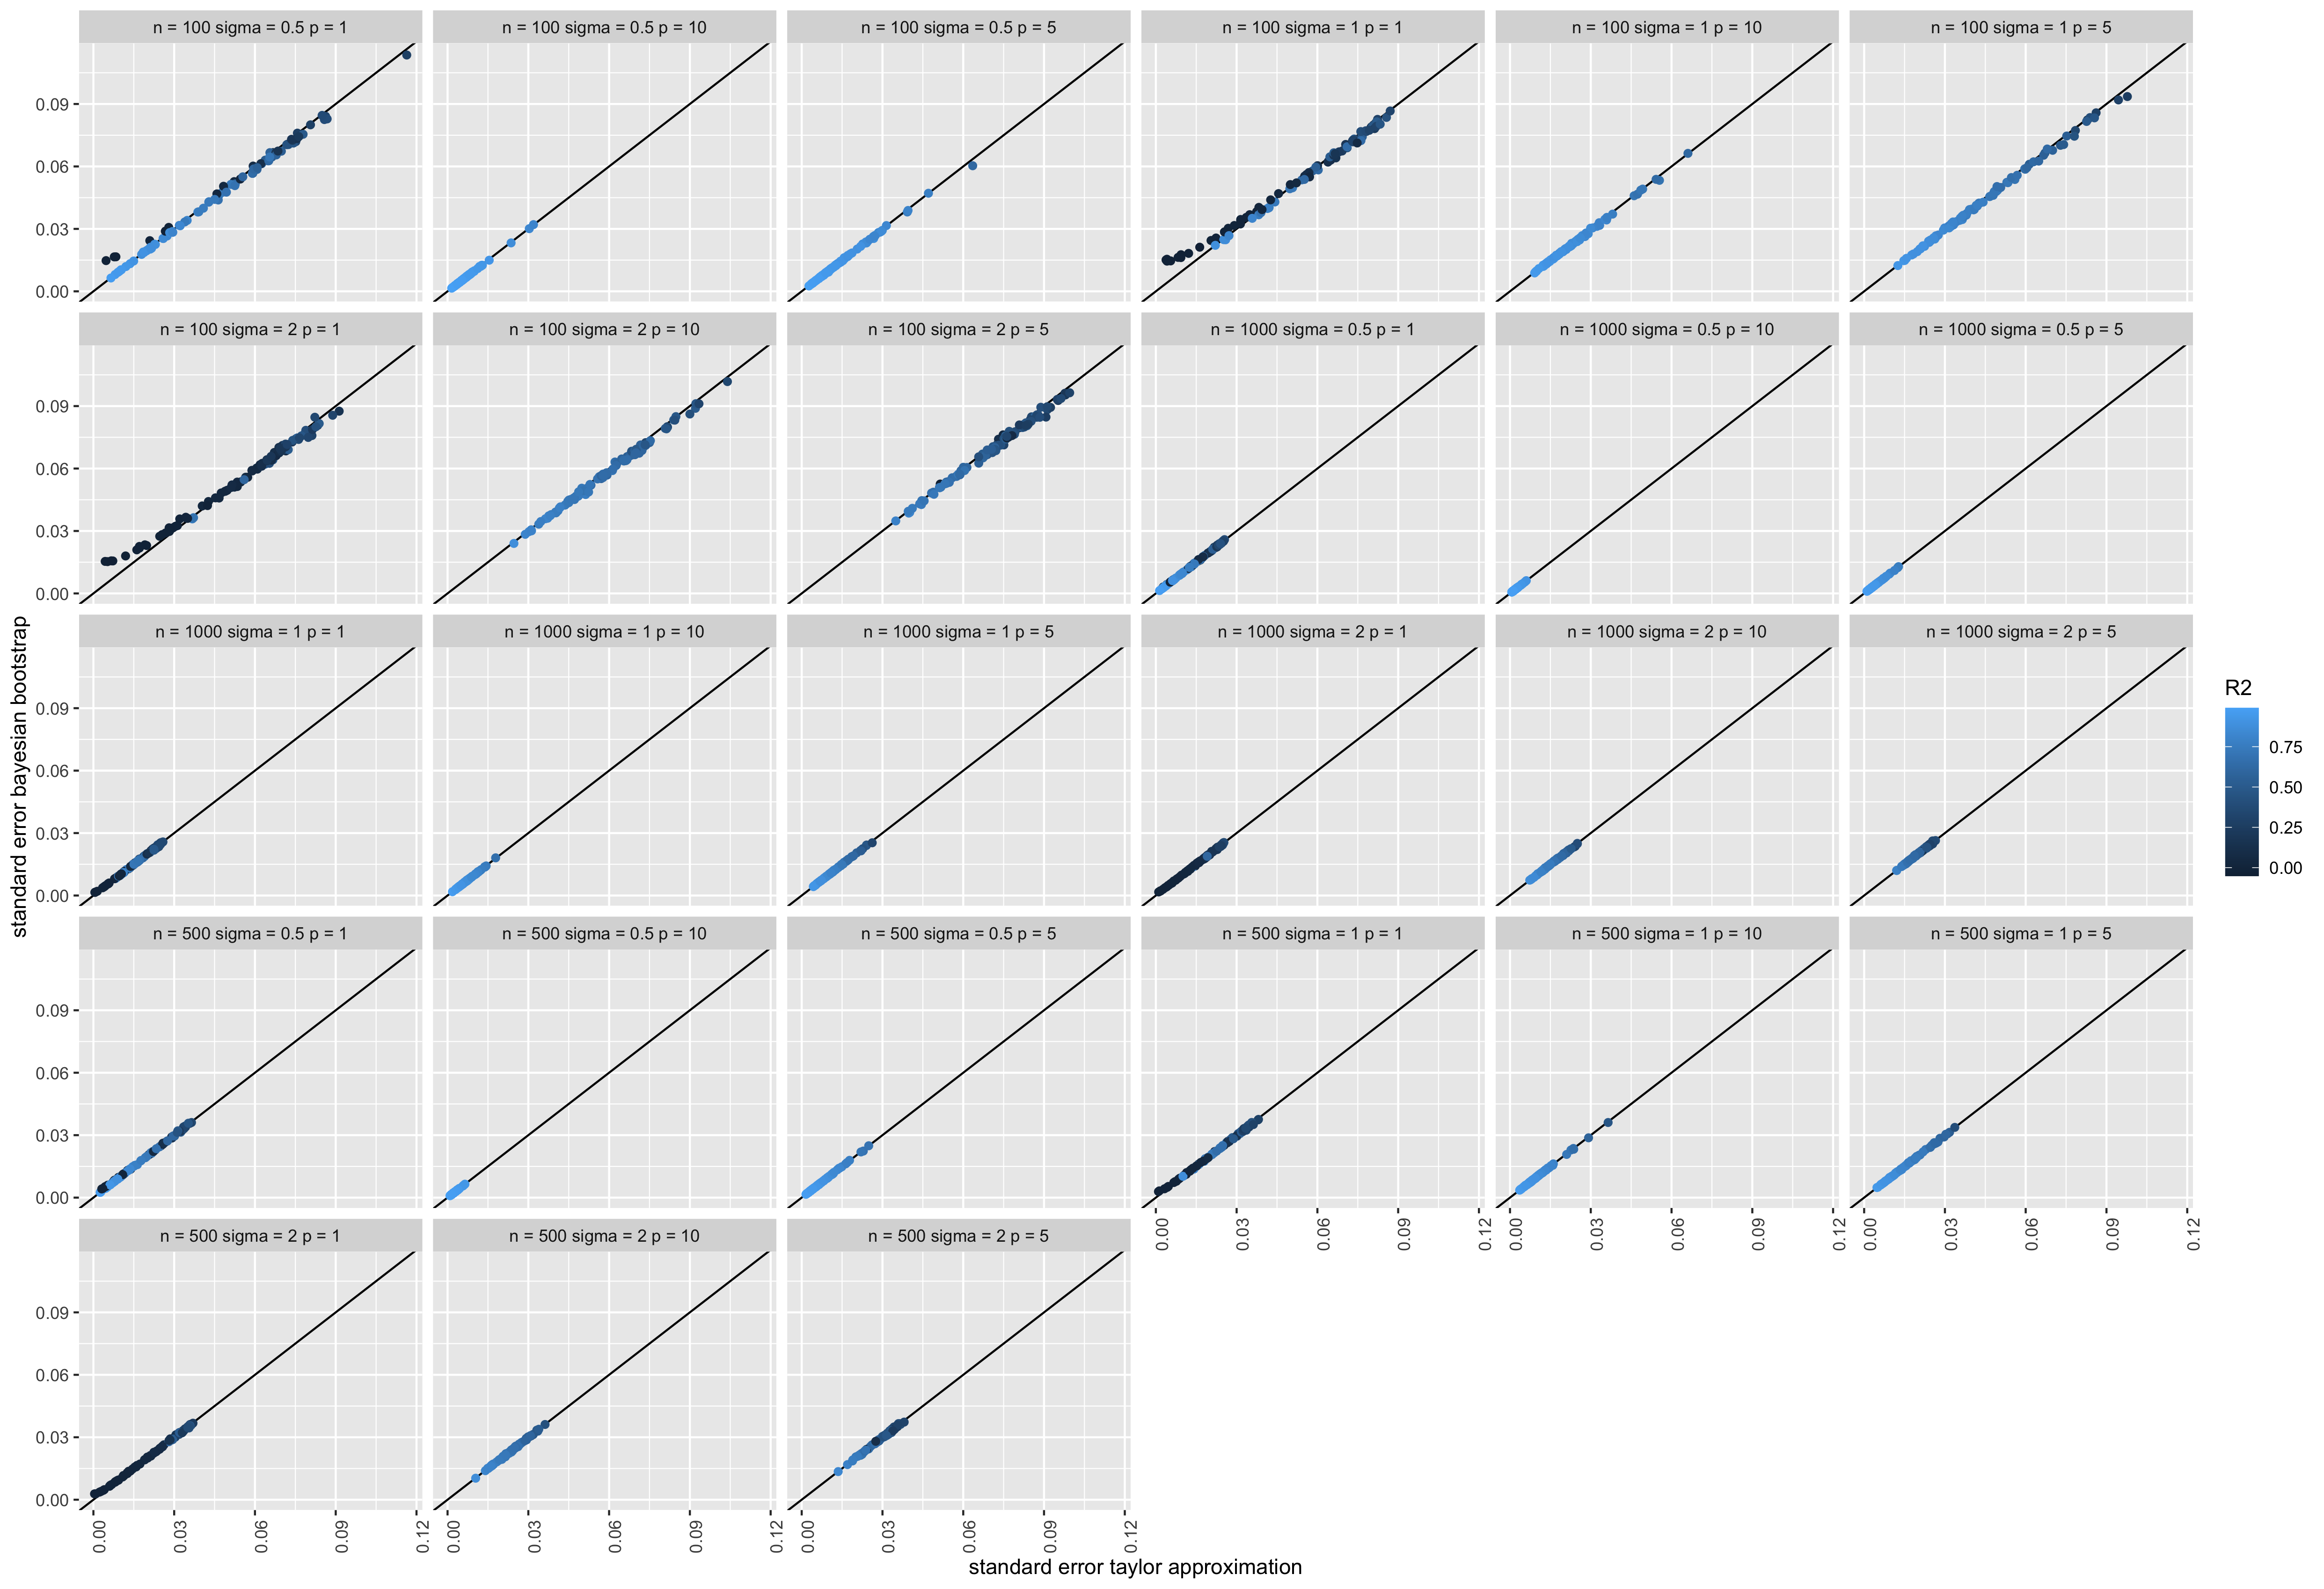
\includegraphics[width=\paperwidth, height=\textheight]{simres.png}
    \caption{Caption}
    \label{fig:my_label}
\end{figure}

\end{document}